\documentclass[12pt]{article}
\usepackage[utf8]{inputenc}
\usepackage[utf8]{inputenc}
\usepackage{amsmath}
\usepackage{amsthm}
\usepackage{geometry}
\usepackage{amsfonts}
\usepackage{mathrsfs}
\usepackage{bm}
\usepackage{hyperref}
\usepackage[dvipsnames]{xcolor}
\usepackage{enumitem}
\usepackage{mathtools}
\usepackage{changepage}
\usepackage{lipsum}
\usepackage{tikz}
\usetikzlibrary{matrix}
\usepackage{tikz-cd}
\usepackage[nameinlink]{cleveref}
\geometry{
headheight=15pt,
left=60pt,
right=60pt
}
\usepackage{fancyhdr}
\pagestyle{fancy}
\fancyhf{}
\lhead{}
\chead{Section 2.5 Exercises}
\rhead{\thepage}
\hypersetup{
    colorlinks=true,
    linkcolor=blue,
    urlcolor=blue
}

\theoremstyle{definition}
\newtheorem*{remark}{Remark}

\newtheoremstyle{exercise}
    {}
    {}
    {}
    {}
    {\bfseries}
    {.}
    { }
    {\thmname{#1}\thmnumber{#2}\thmnote{ (#3)}}
\theoremstyle{exercise}
\newtheorem{exercise}{Exercise 2.5.}

\newtheoremstyle{solution}
    {}
    {}
    {}
    {}
    {\itshape\color{magenta}}
    {.}
    { }
    {\thmname{#1}\thmnote{ #3}}
\theoremstyle{solution}
\newtheorem*{solution}{Solution}

\Crefformat{exercise}{#2Exercise 2.5.#1#3}

\newcommand{\setcomp}[1]{#1^{\mathsf{c}}}
\newcommand{\N}{\mathbf{N}}
\newcommand{\Z}{\mathbf{Z}}
\newcommand{\Q}{\mathbf{Q}}
\newcommand{\R}{\mathbf{R}}
\newcommand{\C}{\mathbf{C}}

\DeclarePairedDelimiter\abs{\lvert}{\rvert}
% Swap the definition of \abs* and \norm*, so that \abs
% and \norm resizes the size of the brackets, and the 
% starred version does not.
\makeatletter
\let\oldabs\abs
\def\abs{\@ifstar{\oldabs}{\oldabs*}}
%
\let\oldnorm\norm
\def\norm{\@ifstar{\oldnorm}{\oldnorm*}}
\makeatother

\setlist[enumerate,1]{label={(\alph*)}}

\begin{document}

\section{Section 2.5 Exercises}

Exercises with solutions from Section 2.5 of \hyperlink{ua}{[UA]}.

\begin{exercise}
\label{ex:1}
    Give an example of each of the following, or argue that such a request is impossible.
    \begin{enumerate}
        \item A sequence that has a subsequence that is bounded but contains no subsequence that converges.

        \item A sequence that does not contain 0 or 1 as a term but contains subsequences converging to each of these values.

        \item A sequence that contains subsequences converging to every point in the infinite set
        \[
            \{ 1, 1/2, 1/3, 1/4, 1/5, \ldots \}.
        \]

        \item A sequence that contains subsequences converging to every point in the infinite set
        \[
            \{ 1, 1/2, 1/3, 1/4, 1/5, \ldots \},
        \]
        and no subsequences converging to points outside of this set.
    \end{enumerate}
\end{exercise}

\begin{solution}
    \begin{enumerate}
        \item This is impossible. If a sequence \( (a_n) \) has a bounded subsequence \( (a_{n_k}) \), then by the Bolzano-Weierstrass theorem there must be a convergent sub-subsequence \( (a_{n_{k_l}}) \); this is also a convergent subsequence of the original sequence \( (a_n) \).

        \item Consider the sequence
        \[
            \left( \tfrac{1}{2}, \tfrac{1}{2}, \tfrac{1}{4}, \tfrac{3}{4}, \tfrac{1}{6}, \tfrac{5}{6}, \ldots \right),
        \]
        i.e.\ the sequence \( (a_n) \) given by
        \[
            a_n = \begin{cases}
                \frac{1}{n+1} & \text{if } n \text{ is odd}, \\
                1 - \frac{1}{n} & \text{if } n \text{ is even}.
            \end{cases}
        \]
        Then \( (a_n) \) does not contain 0 or 1 as a term, the subsequence \( (a_{2k - 1}) \) converges to 0, and the subsequence \( (a_{2k}) \) converges to 1.

        \item Consider the following infinite array:
        \[
            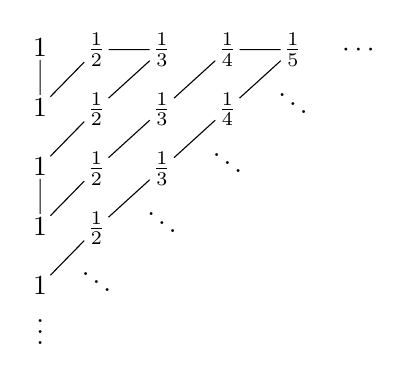
\begin{tikzpicture}
                \matrix[matrix of math nodes,inner sep=1pt,row sep=1pt,column sep=1em] (M)
                {
                    1 & \tfrac{1}{2} & \tfrac{1}{3} & \tfrac{1}{4} & \tfrac{1}{5} & \cdots \\
                    1 & \tfrac{1}{2} & \tfrac{1}{3} & \tfrac{1}{4} & \ddots \\
                    1 & \tfrac{1}{2} & \tfrac{1}{3} & \ddots \\
                    1 & \tfrac{1}{2} & \ddots \\
                    1 & \ddots \\
                    \vdots \\
                }
                ;
                \draw[-] (M-1-1) -- (M-2-1) -- (M-1-2) -- (M-1-3) -- (M-2-2) -- (M-3-1) -- (M-4-1) -- (M-3-2) -- (M-2-3) -- (M-1-4) -- (M-1-5) -- (M-2-4) -- (M-3-3) -- (M-4-2) -- (M-5-1);
            \end{tikzpicture}
        \]
        Let \( (a_n) \) be the sequence obtained by following the lines in the array above;
        \[
            a_1 = 1, a_2 = 1, a_3 = \tfrac{1}{2}, a_4 = \tfrac{1}{3}, a_5 = \tfrac{1}{2}, a_6 = 1, \text{ etc}.
        \]
        Then the subsequence given by the \(n\)th column is \( (1/n, 1/n, 1/n, \ldots) \) and hence converges to \( 1/n \).

        \item This is impossible. Suppose that \( (a_n) \) is a sequence that contains subsequences converging to every point in the infinite set
        \[
            \{ 1, 1/2, 1/3, 1/4, 1/5, \ldots \}.
        \]
        We claim that \( (a_n) \) must have a subsequence converging to 0. We will construct this subsequence inductively as follows. Since there is a subsequence converging to 1, there must be some index \( n_1 \) such that
        \[
            \abs{a_{n_1} - 1} < 1 \iff 0 < a_{n_1} < 2.
        \]
        Since there is a subsequence converging to \( 1/2 \), there must be some index \( n_2 > n_1 \) such that
        \[
            \abs{a_{n_2} - \tfrac{1}{2}} < \tfrac{1}{2} \iff 0 < a_{n_2} < 1.
        \]
        We continue in this manner, obtaining a subsequence \( (a_{n_k}) \) satisfying \( 0 < a_{n_k} < \tfrac{2}{k} \). The Squeeze Theorem then implies that \( \lim_{k \to \infty} a_{n_k} = 0 \).
    \end{enumerate}
\end{solution}

\begin{exercise}
\label{ex:2}
    Decide whether the following propositions are true or false, providing a short justification for each conclusion.
    \begin{enumerate}
        \item If every proper subsequence of \( (x_n) \) converges, then \( (x_n) \) converges as well.

        \item If \( (x_n) \) contains a divergent subsequence, then \( (x_n) \) diverges.

        \item If \( (x_n) \) is bounded and diverges, then there exist two subsequences of \( (x_n) \) that converge to different limits.

        \item If \( (x_n) \) is monotone and contains a convergent subsequence, then \( (x_n) \) converges.
    \end{enumerate}
\end{exercise}

\begin{solution}
    \begin{enumerate}
        \item This is true. By assumption, the subsequence \( (x_2, x_3, x_4, \ldots) \) converges. It is then clear that \( (x_n) \) also converges to the same limit.

        \item This is true. Consider the contrapositive statement: if \( (x_n) \) converges, then all subsequences of \( (x_n) \) converge. This is implied by Theorem 2.5.2.

        \item This is true. Consider the sequences
        \[
            y_n = \sup \{ x_m : m \geq n \} \quad \text{and} \quad z_n = \inf \{ x_m : m \geq n \}.
        \]
        As shown in \href{https://lew98.github.io/Mathematics/UA_Section_2_4_Exercises.pdf}{Exercise 2.4.7}, these sequences both converge since \( (x_n) \) is bounded and their limits are denoted by
        \[
            \limsup x_n = \lim y_n \quad \text{and} \quad \liminf x_n = \lim z_n.
        \]
        It was also shown in that exercise that \( \liminf x_n < \limsup x_n \) since \( (x_n) \) is divergent. We claim that there are subsequences of \( (x_n) \) converging to \( \limsup x_n \) and \( \liminf x_n \). First, we will inductively construct a subsequence converging to \( \limsup x_n \). By the approximation property for suprema, there exists an \( n_1 \geq 1 \) such that \( y_1 - 1 < x_{n_1} \leq y_1 \). There then exists an \( n_2 \geq n_1 + 1 \) such that \( y_{n_1 + 1} - \tfrac{1}{2} < x_{n_2} \leq y_{n_1 + 1} \). Continuing in this fashion, we obtain indices \( n_1 < \cdots < n_k < \cdots \) such that \( y_{n_{k-1} + 1} - \tfrac{1}{k} < x_{n_k} \leq y_{n_{k-1} + 1} \). By Theorem 2.5.2, the subsequence \( (y_{n_{k-1} + 1}) \) converges to \( \limsup x_n \) and hence by the Squeeze Theorem the subsequence \( (x_{n_k}) \) converges to \( \limsup x_n \). Similarly, we can obtain another subsequence converging to \( \liminf x_n \), which is strictly less than \( \limsup x_n \).

        \item This is true. Suppose that \( (x_n) \) is decreasing; the case where \( (x_n) \) is increasing is handled similarly. By assumption, there is a convergent subsequence \( (x_{n_k}) \) which must also be decreasing. By the Monotone Convergence Theorem and the uniqueness of limits, we must have
        \[
            \lim_{k \to \infty} x_{n_k} = x = \inf \{ x_{n_k} : k \in \N \}.
        \]
        Let \( \epsilon > 0 \) be given. There is a \( K \in \N \) such that \( k \geq K \implies \abs{x_{n_k} - x} < \epsilon \). Suppose that \( n \in \N \) is such that \( n \geq n_K \). Then since \( (x_n) \) is decreasing, we have \( x_n \leq x_{n_K} < x + \epsilon \). We claim that \( x_n \geq x \). To see this, suppose that \( x_n < x \). Then since \( (x_{n_k}) \) is a subsequence of the decreasing sequence \( (x_n) \), there must be some \( k \in \N \) such that \( x_{n_k} \leq x_n < x \); but this contradicts that \( x \) is the infimum of \( \{ x_{n_k} : k \in \N \} \). So we have \( x \leq x_n < x + \epsilon \implies \abs{x_n - x} < \epsilon \) and hence
        \[
            n \geq n_K \implies \abs{x_n - x} < \epsilon.
        \]
        It follows that \( \lim_{n \to \infty} x_n = x \).
    \end{enumerate}
\end{solution}

\begin{exercise}
\label{ex:3}
    \begin{enumerate}
        \item Prove that if an infinite series converges, then the associative property holds. Assume \( a_1 + a_2 + a_3 + a_4 + a_5 + \cdots \) converges to a limit \( L \) (i.e., the sequence of partial sums \( (s_n) \to L \)). Show that any regrouping of the terms
        \[
            (a_1 + a_2 + \cdots + a_{n_1}) + (a_{n_1 + 1} + \cdots + a_{n_2}) + (a_{n_2 + 1} + \cdots + a_{n_3}) + \cdots
        \]
        leads to a series that also converges to \( L \).

        \item Compare this result to the example discussed at the end of Section 2.1 where infinite addition was shown not to be associative. Why doesn't our proof in (a) apply to this example?
    \end{enumerate}
\end{exercise}

\begin{solution}
    \begin{enumerate}
        \item We have indices \( n_1 < \cdots < n_k < \cdots \) and we want to show that the series \( \sum_{k=1}^{\infty} b_k = L \), where \( b_1 = a_1 + \cdots + a_{n_1} = s_{n_1} \) and
        \[
            b_k = a_{n_{k-1} + 1} + \cdots + a_{n_k} = s_{n_k} - s_{n_{k-1}}
        \]
        for \( k \geq 2 \). Observe that for \( m \geq 2 \), the partial sums are
        \[
            t_m = \sum_{k=1}^m b_k = s_{n_1} + \sum_{k=2}^m (s_{n_k} - s_{n_{k-1}}) = s_{n_1} + (s_{n_2} - s_{n_1}) + \cdots + (s_{n_m} - s_{n_{m-1}}) = s_{n_m}.
        \]
        Hence by Theorem 2.5.2 we have \( \sum_{k=1}^{\infty} b_k = \lim_{m \to \infty} t_m = \lim_{m \to \infty} s_{n_m} = L \).

        \item Our proof does not apply to the series \( \sum_{n=1}^{\infty} (-1)^n \) since this series does not converge; the sequence of partial sums is \( (-1, 0, -1, 0, \ldots) \).
    \end{enumerate}
\end{solution}

\begin{exercise}
\label{ex:4}
    The Bolzano-Weierstrass Theorem is extremely important, and so is the strategy employed in the proof. To gain some more experience with this technique, assume the Nested Interval Property is true and use it to provide a proof of the Axiom of Completeness. To prevent the argument from being circular, assume also that \( (1/2^n) \to 0 \). (Why precisely is this last assumption needed to avoid circularity?)
\end{exercise}

\begin{solution}
    Let \( E \subseteq \R \) be non-empty and bounded above by some \( b_1 \in \R \). We will show that \( \sup E \) exists. If \( E \) has a maximum \( x \), then \( \sup E = x \) and we are done. Otherwise, we shall use an induction argument to construct a sequence \( (I_n)_{n \in \N} \) of nested intervals. Pick some \( a_1 \in E \); it must be the case that \( a_1 \) is not an upper bound of \( E \) since \( E \) has no maximum. Let \( I_1 = [a_1, b_1] \). Then:
    \begin{itemize}
        \item \( a_1 \) is not an upper bound of \( E \);
        \item \( b_1 \) is an upper bound of \( E \);
        \item \( \abs{I_1} = 2^0 (b_1 - a_1) \).
    \end{itemize}
    Suppose that after \( N \) steps we have chosen intervals \( I_n = [a_n, b_n] \), \( 1 \leq n \leq N \), such that
    \begin{itemize}
        \item \( a_1 \leq \cdots \leq a_N \) are not upper bounds of \( E \);
        \item \( b_N \leq \cdots \leq b_1 \) are upper bounds of \( E \);
        \item \( \abs{I_n} = 2^{-(n-1)}(b_1 - a_1) \) for \( 1 \leq n \leq N \).
    \end{itemize}
    Let \( m = \tfrac{a_N + b_N}{2} \), the midpoint of the interval \( I_N \). If \( m \) is not an upper bound of \( E \), set
    \[
        a_{N+1} = m, b_{N+1} = b_N, \text{and } I_{N+1} = [a_{N+1}, b_{N+1}].
    \]
    If \( m \) is an upper bound of \( E \), set
    \[
        a_{N+1} = a_N, b_{N+1} = m, \text{and } I_{N+1} = [a_{N+1}, b_{N+1}].
    \]
    In either case, we have chosen intervals \( I_n = [a_n, b_n] \), \( 1 \leq n \leq N + 1 \), such that
    \begin{itemize}
        \item \( a_1 \leq \cdots \leq a_{N+1} \) are not upper bounds of \( E \);
        \item \( b_{N+1} \leq \cdots \leq b_1 \) are upper bounds of \( E \);
        \item \( \abs{I_n} = 2^{-(n-1)}(b_1 - a_1) \) for \( 1 \leq n \leq N + 1 \).
    \end{itemize}
    In this way we obtain a sequence \( (I_n)_{n \in \N} \) of intervals \( I_n = [a_n, b_n] \) such that
    \begin{itemize}
        \item \( a_1 \leq \cdots \leq a_n \leq \cdots \) are not upper bounds of \( E \);
        \item \( \cdots \leq b_n \leq \cdots \leq b_1 \) are upper bounds of \( E \);
        \item \( \abs{I_n} = 2^{-(n-1)}(b_1 - a_1) \) for all \( n \in \N \).
    \end{itemize}
    Hence \( (I_n)_{n \in \N} \) is a sequence of nested intervals. By assumption, \( \R \) has the nested interval property, so there exists an \( x \in \R \) such that \( x \in \bigcap_{n=1}^{\infty} I_n \). We claim that \( x = \sup E \). For \( y \in E \), suppose \( x < y \). Since \( \abs{I_n} = 2^{-(n-1)}(b_1 - a_1) \) for all \( n \in \N \) and \( (2^{-n}) \to 0 \) (by assumption), there must exist an \( N \in \N \) such that
    \[
        \abs{I_N} = b_N - a_N < y - x \implies x + (b_N - a_N) < y.
    \]
    Since \( x \in \bigcap_{n=1}^{\infty} I_n \), we have
    \[
        a_N \leq x \implies 0 \leq x - a_N \implies b_N \leq x + (b_N - a_N) < y.
    \]
    This is a contradiction since \( b_N \) is an upper bound of \( E \). It follows that \( y \leq x \), so that \( x \)  is an upper bound of \( E \). Suppose that \( z \in \R \) is such that \( z < x \). Then there must be an \( N \in \N \) such that
    \[
        b_N - a_N < x - z \implies z < x - (b_N - a_N).
    \]
    Since \( x \in \bigcap_{n=1}^{\infty} I_n \), we have
    \[
        x \leq b_N \implies x - b_N \leq 0 \implies x - (b_N - a_N) \leq a_N \implies z < a_N.
    \]
    It follows that \( z \) is not an upper bound of \( E \) since \( a_N \) is not an upper bound of \( E \). We may conclude that \( x \) is the least upper bound of \( E \), i.e.\ \( x = \sup E \).

    We had to assume that \( (1/2^n) \to 0 \) since the usual proof of this would involve the Axiom of Completeness (assume \( A = \{ 2^n : n \in \N \} \) is bounded in \( \R \), invoke AoC to obtain \( \sup A \in \R \), derive contradiction).
\end{solution}

\begin{exercise}
\label{ex:5}
    Assume \( (a_n) \) is a bounded sequence with the property that every convergent subsequence of \( (a_n) \) converges to the same limit \( a \in \R \). Show that \( (a_n) \) must converge to \( a \).
\end{exercise}

\begin{solution}
    Since \( (a_n) \) is bounded, \( \limsup a_n \) and \( \liminf a_n \) are both real numbers. In the solution to \Cref{ex:2} (c), we showed that there are subsequences \( (a_{n_k}) \) and \( (a_{m_k}) \) such that
    \[
        \lim_{k \to \infty} a_{n_k} = \limsup a_n \quad \text{and} \quad \lim_{k \to \infty} a_{m_k} = \liminf a_n.
    \]
    By assumption we have \( \lim_{k \to \infty} a_{n_k} = \lim_{k \to \infty} a_{m_k} = a \) and so by uniqueness of limits we have \( \limsup a_n = \liminf a_n = a \). \href{https://lew98.github.io/Mathematics/UA_Section_2_4_Exercises.pdf}{Exercise 2.4.7} then implies that \( \lim a_n = a \).
\end{solution}

\begin{exercise}
\label{ex:6}
    Use a similar strategy to the one in Example 2.5.3 to show \( \lim b^{1/n} \) exists for all \( b \geq 0 \) and find the value of the limit. (The results in \href{https://lew98.github.io/Mathematics/UA_Section_2_3_Exercises.pdf}{Exercise 2.3.1} may be assumed.)
\end{exercise}

\begin{solution}
    If \( b = 0 \) then \( b^{1/n} = 0 \) for any \( n \in \N \), so \( \lim_{n \to \infty} b^{1/n} = 0 \). Suppose that \( b > 0 \). If \( 0 < b < 1 \), then
    \[
        b < b^{1/2} < b^{1/3} < \cdots < 1.
    \]
    If \( b \geq 1 \), then
    \[
        b \geq b^{1/2} \geq b^{1/3} \geq \cdots \geq 1.
    \]
    In either case, \( (b^{1/n}) \) is bounded and monotone and hence convergent by the Monotone Convergence Theorem, say \( \lim b^{1/n} = l \in \R \). Then by Theorem 2.5.2, we have \( \lim b^{1/2n} = l \) also. Note that
    \[
        \lim b^{1/2n} = \lim \sqrt{b^{1/n}} = \sqrt{\lim b^{1/n}} = \sqrt{l}
    \]
    by \href{https://lew98.github.io/Mathematics/UA_Section_2_3_Exercises.pdf}{Exercise 2.3.1}. Since limits are unique, we must have \( l = \sqrt{l} \), which implies that \( l = 0 \) or \( l = 1 \). If \( 0 < b < 1 \) then the Order Limit Theorem gives \( 0 < b < l \leq 1 \), so we must have \( l = 1 \). If \( b \geq 1 \) then the Order Limit Theorem gives \( l \geq 1 \) so again we must have \( l = 1 \).

    We may conclude that \( \lim b^{1/n} = 0 \) if \( b = 0 \) and \( \lim b^{1/n} = 1 \) if \( b > 0 \).
\end{solution}

\begin{exercise}
\label{ex:7}
    Extend the result proved in Example 2.5.3 to the case \( \abs{b} < 1 \); that is, show \( \lim (b^n) = 0 \) if and only if \( -1 < b < 1 \).
\end{exercise}

\begin{solution}
    We will consider the following cases.
    \begin{itemize}
        \item \( b > 1 \). Then \( (b^n) \) is unbounded and hence divergent.

        \item \( b = 1 \). Then \( (b^n) = (1, 1, 1, \ldots) \) and hence \( \lim b^n = 1 \).

        \item \( 0 < b < 1 \). Example 2.5.3 shows that in this case we have \( \lim b^n = 0 \).

        \item \( b = 0 \). Clearly \( \lim b^n = 0 \).

        \item \( -1 < b < 0 \). Observe that \( b = (-1) \abs{b} \), so that \( b^n = (-1)^n \abs{b}^n \). Since \( 0 < \abs{b} < 1 \), we have \( \lim \abs{b}^n = 0 \) by the \( 0 < b < 1 \) case. Then since \( (-1)^n \) is bounded, we must have
        \[
            \lim b^n = \lim [(-1)^n \abs{b}^n] = 0
        \]
        by \href{https://lew98.github.io/Mathematics/UA_Section_2_3_Exercises.pdf}{Exercise 2.3.9} (a).

        \item \( b = -1 \). Then \( b^n = (-1)^n \), which is divergent since it has two convergent subsequences with different limits:
        \[
            \lim [(-1)^{2n}] = 1 \neq -1 = \lim [(-1)^{2n+1}].
        \]

        \item \( b < -1 \). We have \( b^n = (-1)^n \abs{b}^n \) with \( \abs{b} > 1 \). Observe that the subsequence \( (b^{2n}) = ([\abs{b}^2]^n) \) is divergent by the \( b > 1 \) case. Then the sequence \( (b^n) \) itself is divergent by \Cref{ex:2} (b).
    \end{itemize}
    We may conclude that \( \lim b^n = 0 \) if and only if \( -1 < b < 1 \).
\end{solution}

\begin{exercise}
\label{ex:8}
    Another way to prove the Bolzano-Weierstrass Theorem is to show that every sequence contains a monotone subsequence. A useful device in this endeavor is the notion of a \textit{peak term}. Given a sequence \( (x_n) \), a particular term \( x_m \) is a peak term if no later term in the sequence exceeds it; i.e., if \( x_m \geq x_n \) for all \( n \geq m \).
    \begin{enumerate}
        \item Find examples of sequences with zero, one, and two peak terms. Find an example of a sequence with infinitely many peak terms that is not monotone.

        \item Show that every sequence contains a monotone subsequence and explain how this furnishes a new proof of the Bolzano-Weierstrass Theorem.
    \end{enumerate}
\end{exercise}

\begin{solution}
    \begin{enumerate}
        \item Any strictly increasing sequence will have zero peak terms; the sequence \( (n) \) for example. For sequences with one and two peak terms, consider (respectively)
        \[
            \left(2, 0, \tfrac{1}{2}, \tfrac{2}{3}, \tfrac{3}{4}, \tfrac{4}{5}\ldots\right) \quad \text{and} \quad \left(3, 2, 0, \tfrac{1}{2}, \tfrac{2}{3}, \tfrac{3}{4}, \tfrac{4}{5}\ldots\right).
        \]
        For a sequence with infinitely many peak terms but which is not monotone, consider
        \[
            (0, 1, -2, -1, -4, -3, \ldots).
        \]

        \item Let \( (x_n) \) be a sequence; we will show that \( (x_n) \) contains a monotone subsequence. First, suppose that \( (x_n) \) contains infinitely many peak terms, say \( x_{n_1}, x_{n_2}, \ldots, x_{n_k}, \ldots \), where we may assume that \( n_1 < n_2 < \cdots < n_k < \cdots \); the subsequence \( (x_{n_k}) \) is then a decreasing subsequence of \( (x_n) \). Next, suppose that \( (x_n) \) contains only finitely many peak terms. In this case, we are guaranteed the existence of a term \( x_{n_1} \) which is not a peak term and after which there are no peak terms. Since \( x_{n_1} \) is not a peak term, there exists \( n_2 > n_1 \) such that \( x_{n_2} > x_{n_1} \) and \( x_{n_2} \) is not a peak term. Then since \( x_{n_2} \) is not a peak term, there exists \( n_3 > n_2 \) such that \( x_{n_3} > x_{n_2} \) and \( x_{n_3} \) is not a peak term. Continuing in this way, we inductively obtain an increasing subsequence \( (x_{n_k}) \) of \( (x_n) \). In either case, we have shown that \( (x_n) \) must contain a monotone subsequence.

        Now suppose that \( (x_n) \) is a bounded sequence. By the previous paragraph, there exists a monotone subsequence \( (x_{n_k}) \), which must also be bounded. The Monotone Convergence Theorem then implies that \( (x_{n_k}) \) is convergent; this provides another proof of the Bolzano-Weierstrass Theorem.
    \end{enumerate}
\end{solution}

\begin{exercise}
\label{ex:9}
    Let \( (a_n) \) be a bounded sequence, and define the set
    \[
        S = \{ x \in \R : x < a_n \text{ for infinitely many terms } a_n \}.
    \]
    Show that there exists a subsequence \( (a_{n_k}) \) converging to \( s = \sup S \). (This is a direct proof of the Bolzano-Weierstrass Theorem using the Axiom of Completeness.)
\end{exercise}

\begin{solution}
    Since \( (a_n) \) is bounded, there is an \( M > 0 \) such that \( -M \leq a_n \leq M \) for all \( n \in \N \). It follows that \( (-\infty, -M) \subseteq S \), so that \( S \) is non-empty, and for any \( x \in S \) we have \( x < a_n \leq M \) for some \( n \in \N \), so that \( S \) is bounded above by \( M \). The Axiom of Completeness then implies that \( s := \sup S \) exists in \( \R \).

    Let \( k \) be a positive integer. We claim that the set
    \[
        B_k = \left\{ n \in \N : s - \tfrac{1}{k} < a_n \leq s + \tfrac{1}{k} \right\}
    \]
    is infinite. By the approximation property for suprema, there exists an \( x \in S \) such that \( s - \tfrac{1}{k} < x \leq s \). Define the sets
    \[
        E = \{ n \in \N : x < a_n \}, \quad A_k = \left\{ n \in \N : s + \tfrac{1}{k} < a_n \right\} \quad \text{and} \quad B'_k = \left\{ n \in \N : x < a_n \leq s + \tfrac{1}{k} \right\}
    \]
    and observe that \( E \) is the disjoint union of \( A_k \) and \( B'_k \) and that \( E \) is infinite since \( x \in S \). Furthermore, \( A_k \) must be finite, otherwise we would have \( s + \tfrac{1}{k} \in S \). It follows that \( B'_k \) is infinite and hence that \( B_k \) is infinite, since \( B'_k \subseteq B_k \).

    Since \( B_1 \) is infinite, there exists some \( n_1 \in \N \) such that \( s - 1 < a_{n_1} \leq s + 1 \). Then since \( B_2 \) is infinite, there exists some \( n_2 > n_1 \) such that \( s - \tfrac{1}{2} < a_{n_2} \leq s + \tfrac{1}{2} \). We continue this process inductively to obtain a subsequence \( (a_{n_k}) \) satisfying \( s - \tfrac{1}{k} < a_{n_k} \leq s + \tfrac{1}{k} \). The Squeeze Theorem then implies that \( \lim_{k \to \infty} a_{n_k} = s \).
\end{solution}

\noindent \hrulefill

\noindent \hypertarget{ua}{\textcolor{blue}{[UA]} Abbott, S. (2015) \textit{Understanding Analysis.} 2nd edn.}

\end{document}
